\begin{problem}[Primer ejemplo elíptico]

Antes de modificar el programa~\ref{code:elliptic1D.m}, responda las
siguientes preguntas.

\begin{enumerate}
  \item

        ¿Cuál ecuación diferencial se está resolviendo?

        \begin{solution}
          Se está resolviendo un problema de valor de frontera Robin
          de $2$ puntos~\cite{CORBINO2020112326}.
          \begin{equation}\label{eq:poisson1drobindconditions}
            \left\{
            \begin{aligned}
              \diff[2]{u}{x}
               & =e^{x},
              \text{ para }x\in\left[0,1\right].     \\
              0
               & = u\left(0\right)-\diff{u}{x}[x=0]. \\
              2e
               & =u\left(1\right)+\diff{u}{x}[x=1].
            \end{aligned}
            \right.
          \end{equation}
          \noQED
        \end{solution}

  \item

        ¿Cuál es la función de fuerza o lado derecho?

        \begin{solution}
          La función de fuerza es $e^{x}$.
          \noQED
        \end{solution}

  \item

        ¿Cuál es el tipo de condiciones de contorno y cuáles son
        los valores de su lado derecho?

        \begin{solution}
          La condición de contorno es Robin con los
          coeficientes Dirichlet y Neumann iguales a $1$.
          Los valores son $g\left(x=0\right)=0$ y
          $g\left(x=1\right)=2e$.
          \noQED
        \end{solution}

  \item

        ¿Cuál es la solución exacta?

        \begin{solution}
          Integramos dos veces y obtenemos la solución
          general.
          \begin{align*}
            \iint
            \diff[2]{u}{x}
            \dl x
            \dl x           & =
            \iint
            e^{x}
            \dl x
            \dl x.              \\
            \int
            \diff{u}{x}
            \dl x           & =
            \int
            \left(e^{x}+C_{1}\right)
            \dl x.              \\
            u\left(x\right) & =
            e^{x}+C_{1}x+C_{2}.
          \end{align*}
          Ahora, apliquemos las condiciones de frontera Robin.
          \begin{equation}\label{eq:linearsystem}
            \left\{
            \begin{aligned}
              0
               & =
              u\left(0\right)-
              \diff{u}{x}[x=0]=
              e^{0}+C_{1}\left(0\right)+C_{2}-
              \left(e^{0}+C_{1}\right)=
              C_{2}-C_{1}. \\
              2e
               & =
              u\left(1\right)+
              \diff{u}{x}[x=1]=
              e^{1}+C_{1}\left(1\right)+C_{2}+
              \left(e^{1}+C_{1}\right)=
              2e+2C_{1}+C_{2}.
            \end{aligned}
            \right.
          \end{equation}
          El sistema~\eqref{eq:linearsystem} tiene como solución
          $C_{1}=C_{2}=0$.
          $\therefore$ la solución
          de~\eqref{eq:poisson1drobindconditions} es
          $u\left(x\right)=e^{x}$.
          \noQED
        \end{solution}
\end{enumerate}

\section*{Explicación del Programa~\ref{code:elliptic1D.m}} %\textsf{}

\begin{itemize}
  \item

        En la línea $1$ encontramos el
        \emph{shebang}\footnote{\url{https://en.wikipedia.org/wiki/Shebang_(Unix)}},
        esto permite ejecutar un script de Octave
        \mintinline{bash}|./elliptic1D.m| con la opción de modo de
        procesamiento por lotes (batch), para esto se necesita
        tener permisos de ejecución (por ejemplo,
        \mintinline{bash}|chmod +x elliptic1D.m|).

  \item

        En las líneas $2$ al $10$ tenemos un comentario sobre el
        programa de modo que ayude al codificador a obtener un
        contexto del problema a resolver.

  \item

        En la línea $12$, la función
        \href{https://docs.octave.org/v9.3.0/Manipulating-the-Load-Path.html#index-addpath}{\mintinline{octave}|addpath|}
        agrega el directorio
        \mintinline{octave}|"/usr/share/mole/matlab/"| a la ruta de
        búsqueda de la función.
        Allí se encuentran el conjunto de scripts Octave / MATLAB
        de la biblioteca MOLE.
        Vea el Programa~\ref{code:moledirectoriesoctave.txt}.

  \item

        En las líneas $14$ y $15$, se inicializan los identicadores
        \mintinline{octave}|west| (oeste, izquierda),
        \mintinline{octave}|east| (este, derecha) con los valores
        de $0$ y $1$, respectivamente, estos representan los
        valores de frontera del dominio espacial
        en~\eqref{eq:poisson1drobindconditions}.

  \item

        En la línea $21$, llamamos a la función
        \href{https://carlosal1015.github.io/mole_examples/api_docs/matlab/src/matlab/lap.html}{\mintinline{octave}|lap|},
        este genera un operador Laplaciano discreto extendido que
        requiere como argumentos obligatorios el orden de precisión
        \mintinline{octave}|k|, el número  de celdas
        \mintinline{octave}|m| y el tamaño de paso
        \mintinline{octave}|dx|.
        \begin{equation*}
          L=L^{\left(k\right)}=
          D^{\left(k\right)}
          G^{\left(k\right)}=
          DG.\qquad\qquad
          \left(
          \difc.L.{}{}=\nabla\cdot\nabla
          \right),
        \end{equation*}
        donde $D$ y $G$ son los operadores miméticos de divergencia
        y gradiente, respectivamente.
        Dado que
        \begin{math}
          D\in
          \mathbb{R}^{\left(m+2\right)\times\left(m+1\right)}
        \end{math}
        y
        \begin{math}
          G\in
          \mathbb{R}^{\left(m+1\right)\times\left(m+2\right)}
        \end{math},
        entonces
        \begin{math}
          L\in
          \mathbb{R}^{\left(m+2\right)\times\left(m+2\right)}
        \end{math}.

  \item

        En la línea $22$, con la función
        \href{https://docs.octave.org/v9.3.0/Figure-Properties.html#index-figure-visible}{\mintinline{octave}|figure|}
        desactivamos que se muestre la figura en la pantalla,
        preferimos solamente guardar la gráfica.

  \item

        En la línea $23$, con la función
        \href{https://docs.octave.org/latest/Information.html#index-spy}{\mintinline{octave}|spy|}
        graficamos (no se mostrará) el patrón de dispersidad de
        $L$.

        \begin{figure}[ht!]
          \centering
          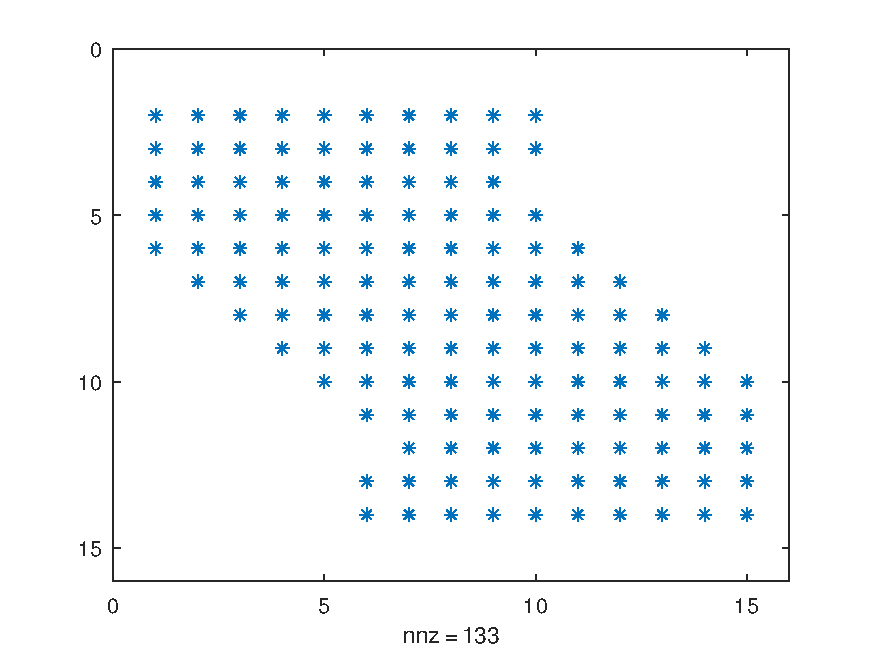
\includegraphics[width=.39\paperwidth]{elliptic1Dsparsebefore.pdf}
          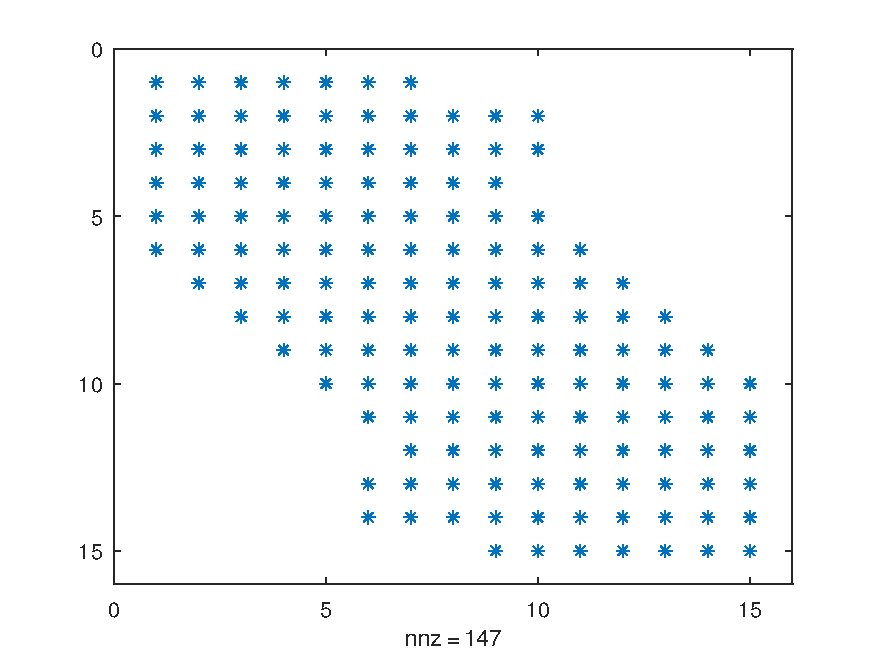
\includegraphics[width=.39\paperwidth]{elliptic1Dsparseafter.pdf}
          \caption{Izquierda: Representación dispersa de $L$ hasta la línea
            21.
            La primera y la última fila son vectores de ceros.
            Derecha: Representación dispersa de $L$ hasta la línea 29.
            La matriz $L\in\mathbb{R}^{15\times 15}$.}
        \end{figure}

  \item

        En la línea $24$, con la función
        \href{https://docs.octave.org/latest/Printing-and-Saving-Plots.html}{\mintinline{octave}|saveas|}
        guardamos esta gráfica en formato PDF y recortado.

  \item

        En la línea $29$, llamamos a la función
        \href{https://carlosal1015.github.io/mole_examples/api_docs/matlab/src/matlab/robinBC.html}{\mintinline{octave}|robinBC|},
        este requiere como argumentos obligatorios el orden de
        precisión \mintinline{octave}|k|, el número  de celdas
        \mintinline{octave}|m|, el tamaño de paso
        \mintinline{octave}|dx|, el coeficiente Dirichlet
        \mintinline{octave}|a| y el coeficiente Neumann
        \mintinline{octave}|b|.
        Esta función devuelve una matriz en
        \begin{math}
          \mathbb{R}^{\left(m+2\right)\times\left(m+2\right)}
        \end{math}.
        Actualizamos la matriz \mintinline{octave}|L| según el
        Algoritmo~\ref{algo:updateL}.

        \begin{algorithm}[H]
          \caption{Actualizaciones del operador Laplaciano discreto extendido.}\label{algo:updateL}
          $A\leftarrow L$\;
          $F\leftarrow f$\;
          $A\leftarrow A+R_{G}$\;
          $U\leftarrow \text{solve}\left(A, F\right)$\;
        \end{algorithm}

  \item

        En la línea $34$, creamos la malla escalonada
        unidimensional, note que los puntos internos son los
        centros de las celdas equiespaciados por
        \mintinline{octave}|dx|.
        La distancia entre el extremo izquierdo y el posterior
        punto malla, así como del extremo derecho y el anterior
        punto malla es \mintinline{octave}|dx/2|.

  \item

        En las líneas $35$ y $43$, guardamos
        \href{https://docs.octave.org/latest/Simple-File-I_002fO.html#index-save-6}{\mintinline{octave}|save|}
        la malla computacional y la solución en el formato HDF5
        para posterior post procesamiento.

  \item

        En la líneas $39$ y $40$, aplicamos las condiciones de
        frontera Robin, empleamos la función
        \href{https://docs.octave.org/latest/Exponents-and-Logarithms.html#XREFexp}{\mintinline{octave}|exp|}.
        El signo menos que antecede al coeficiente Neumann
        \mintinline{octave}|b| se debe a que en el borde izquierdo
        de la malla el vector normal hacia afuera apunta hacia la
        izquierda, mientras que en el borde derecho el vector
        normal hacia afuera apunta hacia la derecha.

  \item

        En la línea $42$, resolvemos el sistema de ecuaciones lineales
        disperso con la función \href{https://docs.octave.org/latest/Arithmetic-Ops.html#index-mldivide}{\mintinline{octave}|mldivide|}.

        \begin{figure}[ht!]
          \centering
          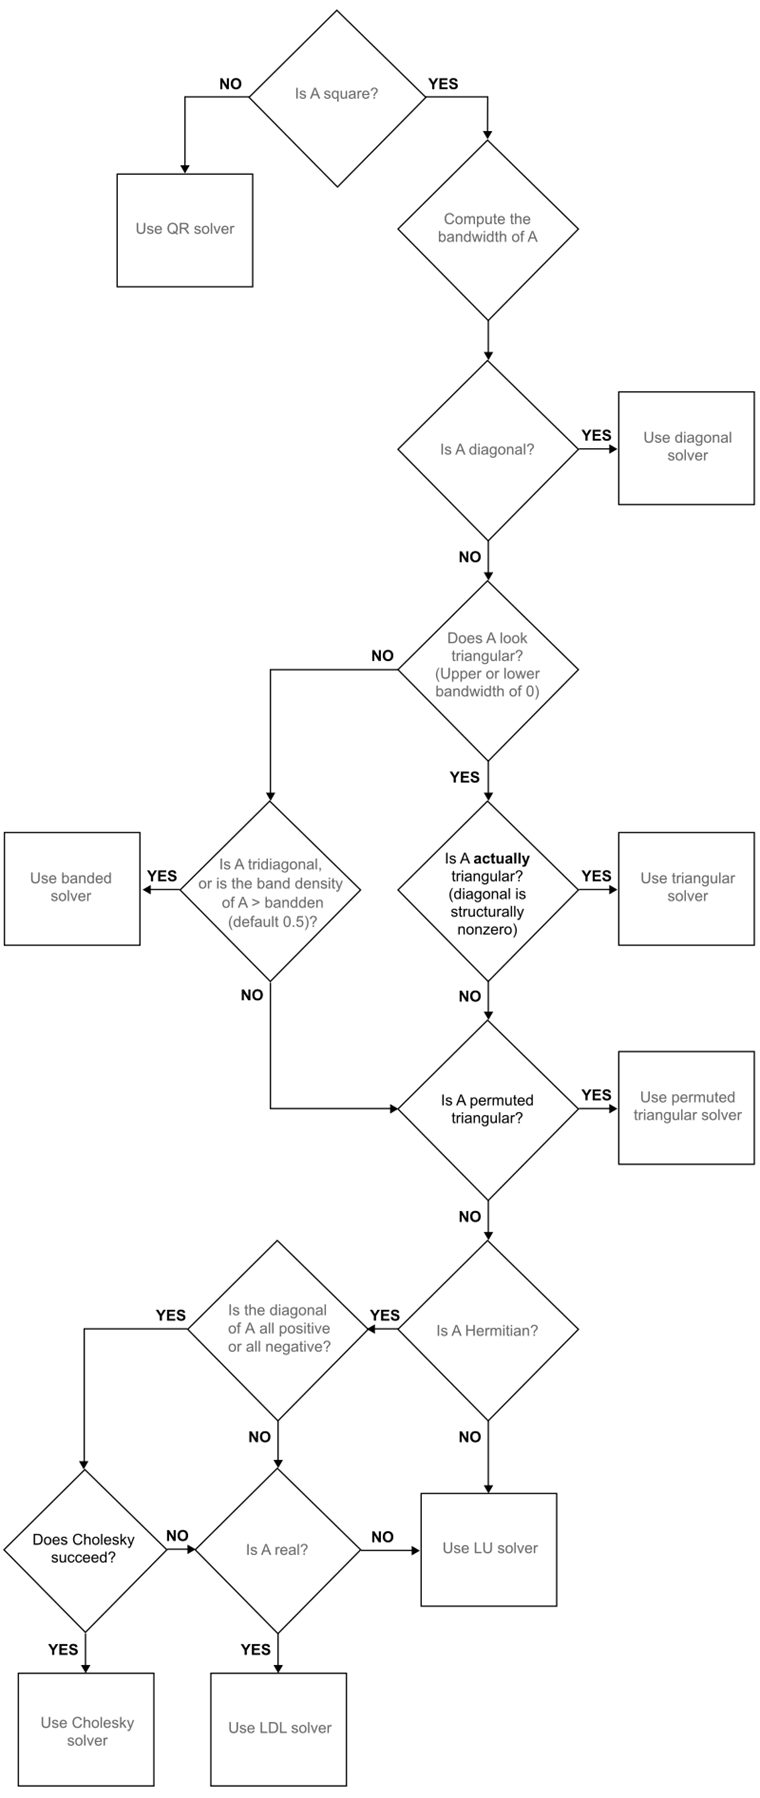
\includegraphics[width=.3\paperwidth]{mldivide_sparse}
          \caption{Diagrama de flujo del solucionador
            \mintinline{octave}|mldivide| para matrices
            disperas que emplea MATLAB.
            Recuperado de~\url{https://www.mathworks.com/help/matlab/ref/double.mldivide.html}.}
        \end{figure}
\end{itemize}

\section*{Resultados del Programa~\ref{code:elliptic1D.m}}

En primer lugar, mostramos la gráfica a escala 1:1 de la solución
exacta y de la solución mimética obtenida en el Programa~\ref{code:elliptic1D.m}.

\begin{figure}[ht!]
  \centering
  % 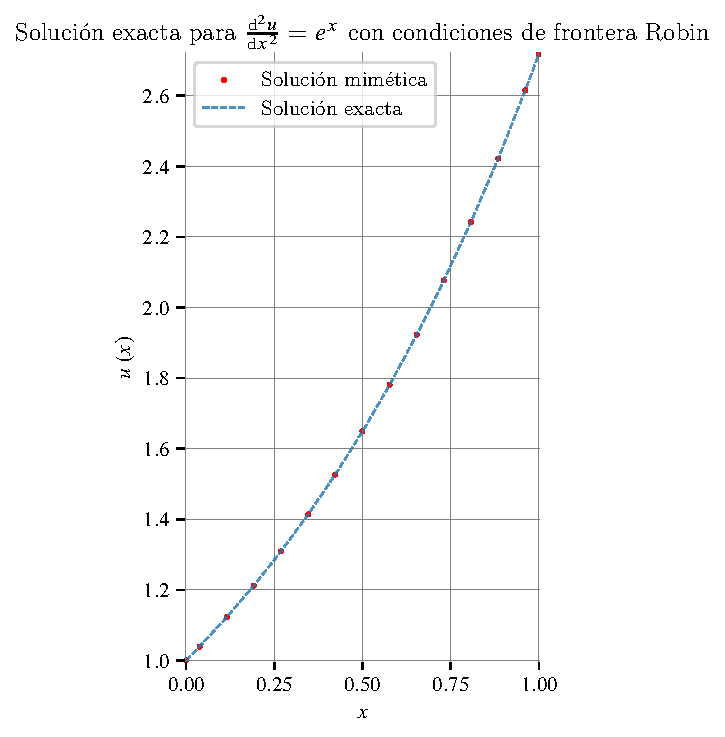
\includegraphics[width=.6\paperwidth]{elliptic1D.pdf}
  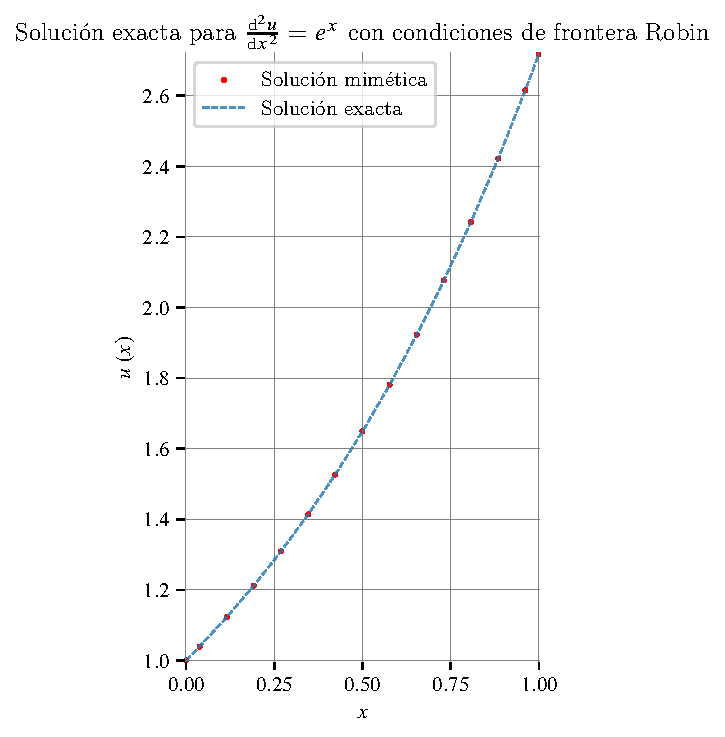
\includegraphics[width=.39\paperwidth]{elliptic1D.pdf}
  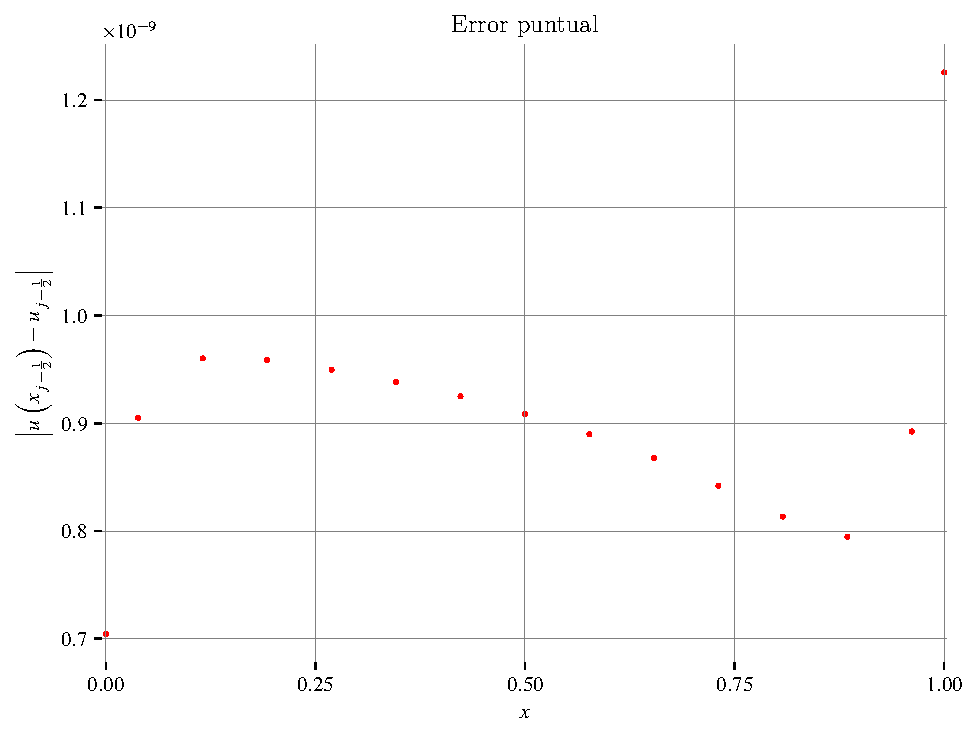
\includegraphics[width=.39\paperwidth]{elliptic1Derror.pdf}
  \caption{Izquierda: Solución de~\eqref{eq:poisson1drobindconditions}
    usando \mintinline{octave}|k=6| y \mintinline{octave}|m=2k+1=13|.
    Derecha: Error en la malla escalonada
    \begin{math}
      \left\{
      0,
      \dotsc,
      x_{j-\frac{1}{2}}
      \dotsc,
      1
      \right\}
    \end{math}}
\end{figure}

En segundo lugar, mostramos una gráfica del error en cada punto de la malla computacional
dada por
\begin{equation*}
  \text{Error de $u$ en $x_{j-\frac{1}{2}}$}=
  \left|
  u\left(x_{j-\frac{1}{2}}\right)-
  u_{j-\frac{1}{2}}
  \right|.
\end{equation*}

Por último, mostramos la tabla de los errores y el orden de convergencia numérico.

\begin{table}[ht!]
  \centering
  \begin{tabular}{ccc}
    \toprule
    $\Delta x$            & Error $\ell_1$        & Orden    \\
    \midrule
    $1.562\times 10^{-2}$ & $4.410\times 10^{-2}$ & -        \\
    $1.535\times 10^{-2}$ & $4.464\times 10^{-2}$ & $-0.678$ \\
    \bottomrule
  \end{tabular}
  \caption{Tabla de errores de aproximación de $U$ en
    $x_{j-\frac{1}{2}}$ y el orden convergencia numérico obtenido.}
  \label{table:errors}
\end{table}

% 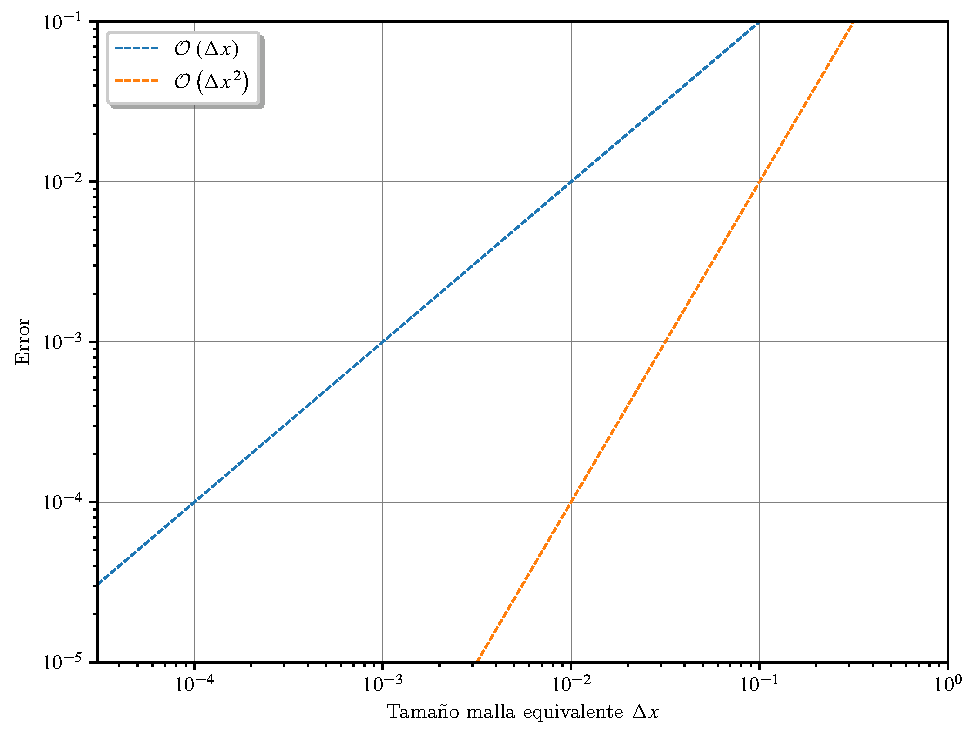
\includegraphics[width=.3\paperwidth]{elliptic1Dconvergenceorder.pdf}
% \DNF<Obtener el orden de convergencia numérico> Abajo: Estimación del orden de convergencia.

\section*{Explicación del Programa~\ref{code:elliptic1D.cpp}}

\begin{itemize}
  \item

        En las tres primeras líneas tenemos un comentario sobre el
        programa de modo que ayude al codificador a obtener un
        contexto del problema a resolver.

  \item

        En la línea $5$
        \href{https://arma.sourceforge.net/docs.html#config_hpp}{\mintinline{cpp}|ARMA_USE_HDF5|}
        para habilitar la lectura y/o escritura de archivos HDF5.

  \item

        En la línea $16$, se inicializa el orden de precisión del
        operador.

  \item

        En las líneas $17$ y $18$, se inicializan los valores que
        representan los bordes del dominio espacial.

  \item

        \mintinline{cpp}|using Real = double| es un alias que se ha
        definido en \mintinline{cpp}|#include <mole/robinbc.h>|.

  \item

        En la línea $23$ se instancia la clase
        \href{https://carlosal1015.github.io/mole_examples/api_docs/cpp/html/classLaplacian.html}{\mintinline{cpp}|Laplacian|}

  \item

        En la línea $26$ se instancia la clase
        \href{https://carlosal1015.github.io/mole_examples/api_docs/cpp/html/classRobinBC.html}{\mintinline{cpp}|RobinBC|}

  \item

        \href{https://arma.sourceforge.net/docs.html#Col}{\mintinline{cpp}|arma::vec|}.

  \item

        .
\end{itemize}
\noQED % Use \noqed or \noQED at the end to suppress the Q.E.D. symbol that marks the end of the current problem.
\end{problem}
